\def\customimage{5em}
\begin{tikzpicture}[node distance = 2]
    \node (P-0) at (0, 0) {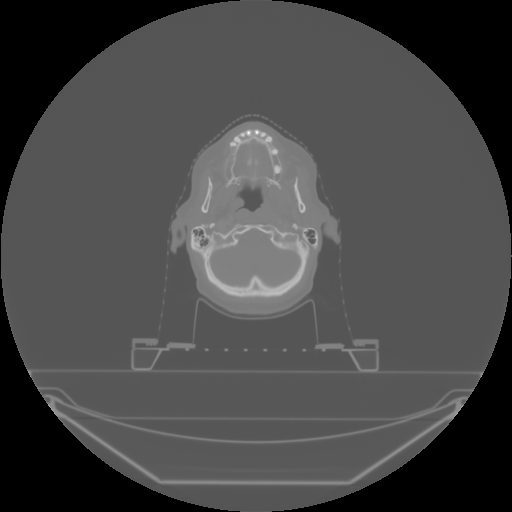
\includegraphics[width=\customimage]{images/preprocess/process_0}};
    \node [below = of P-0] (P-1) {
\includegraphics[width=\customimage]{images/preprocess/process_1}};

    \node [below = .2 of P-0] (text-0) {Scan};
    \node [below = .2 of P-1] (text-1) {Mask};
    
    \node [right = of P-1] (P-2-0) {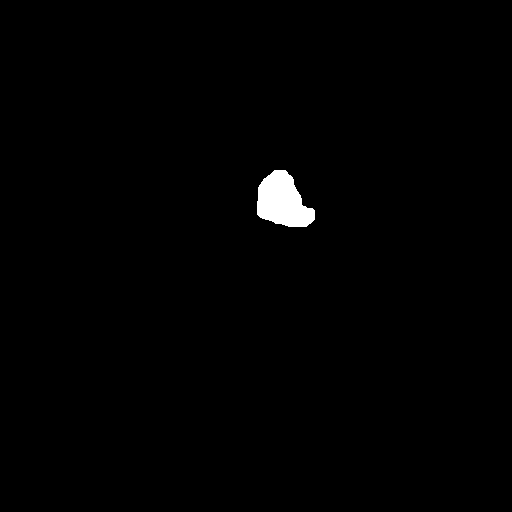
\includegraphics[width=\customimage]{images/preprocess/process_2_0}};
    \node [right = of P-2-0] (P-2-1) {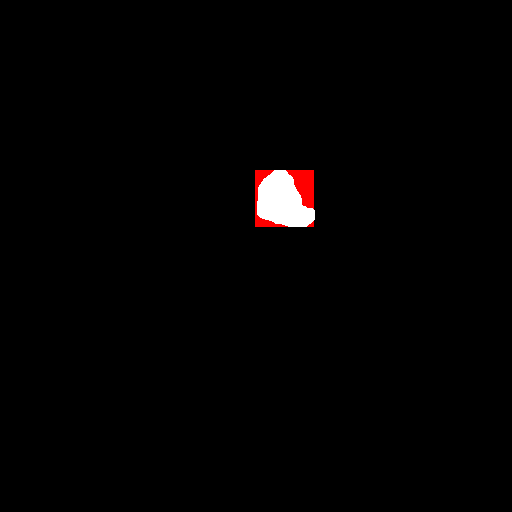
\includegraphics[width=\customimage]{images/preprocess/process_2_1}};
    \node [right = of P-2-1] (P-5) {
\includegraphics[width=\customimage]{images/preprocess/process_5}};
    
    \node [above = of P-2-1] (P-3) {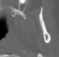
\includegraphics[width=\customimage]{images/preprocess/process_3}};
    \node [right = of P-3] (P-4) {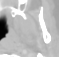
\includegraphics[width=\customimage]{images/preprocess/process_4}};

    \node [right = .5 of P-5, circle, draw] (prod) { \Large \( \times \) };
    
    \node [below = of P-5] (P-6) {
\includegraphics[width=\customimage]{images/preprocess/process_6}};
    \node [left = of P-6] (P-7) {
\includegraphics[width=\customimage]{images/preprocess/process_7}};
    \node [left = of P-7] (P-8) {
\includegraphics[width=\customimage]{images/preprocess/process_8}};

    \node [below = .2 of P-6] { \( 59 \times 57 \) px};
    \node [below = .2 of P-7] { \( 64 \times 64 \) px};
    \node [below = .2 of P-8] { \( 64 \times 64 \) px};

    \draw [-latex] (P-0) -- (P-3);
    \draw [-latex] (P-3) -- (P-4) node[midway, below, align=center] {Remove \\ extreme \\ values};
    \draw [-latex] (P-4) -| (prod);

    \draw [-latex] (P-1) -- (P-2-0) node[midway, below, align=center] {Gaussian \\ filter};
    \draw [-latex] (P-2-0) -- (P-2-1) node[midway, below, align=center] {Bounding \\ box};
    \draw [-latex] (P-2-1) -- (P-3) node[midway, right, align=center] {Slice};
    \draw [-latex] (P-2-1) -- (P-5) node[midway, below, align=center] {Slice};
    \draw [-latex] (P-5) -- (prod);

    \draw [-latex] (prod) |- (P-6) node[near end, below, align=center] {Apply \\ mask};
    \draw [-latex] (P-6) -- (P-7) node[midway, below, align=center] {
        Resize \\ \( 64 \times 64 \)
    };

    \draw [-latex] (P-7) -- (P-8) node[midway, below, align=center] {Normalize};

\end{tikzpicture}